\section{1174009 - Dwi Yulianingsih}
\subsection{Teori}
\begin{enumerate}
\item Kenapa file Text harus di Tokenizer
\par Tokenizer adalah langkah pertama yang diperlukan dalam tugas pemrosesan bahasa, seperti penghitungan kata, penguraian, pemeriksaan ejaan, pembuatan corpus, dan analisis statistik teks. Itu mengkonversi string teks Python menjadi aliran objek token, di mana setiap objek token adalah kata yang terpisah, tanda baca, nomor / jumlah, tanggal, email, URL / URI, dll. Ini juga mengelompokkan aliran token menjadi kalimat, dengan mempertimbangkan sudut kasus-kasus seperti singkatan dan tanggal di tengah kalimat. ilustrasi dapat dilihat pada gambar

\begin{figure}[H]
    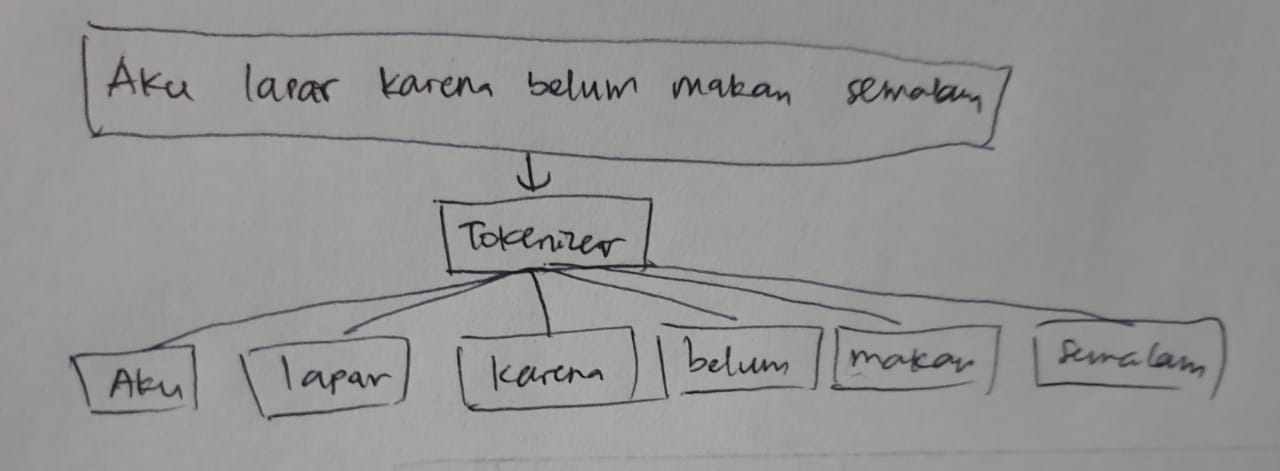
\includegraphics[width=4cm]{figures/1174009/chapter7/teori1.jpeg}
    \centering
      \caption{Ilustrasi Tokenisasi}
\end{figure}

\item Konsep dasar K Fold Cross Validation pada dataset Komentar Youtube

\begin{lstlisting}[caption=K Fold Cross Validation,label={lst:1}]
kfold = StratifiedKFold(n_splits=5)
splits = kfold.split(d, d['CLASS'])
\end{lstlisting}

\par pada Code pada Listing \ref{lst:1} terdapat penggunaan K Fold dengan metode yang akan membagi data dalam 5 hasil pengulangan dari pembagian data yang akan dilakukan pada Attribute CLASS. ilustrasinya dapat dilihat pada Gambar

\begin{figure}[H]
    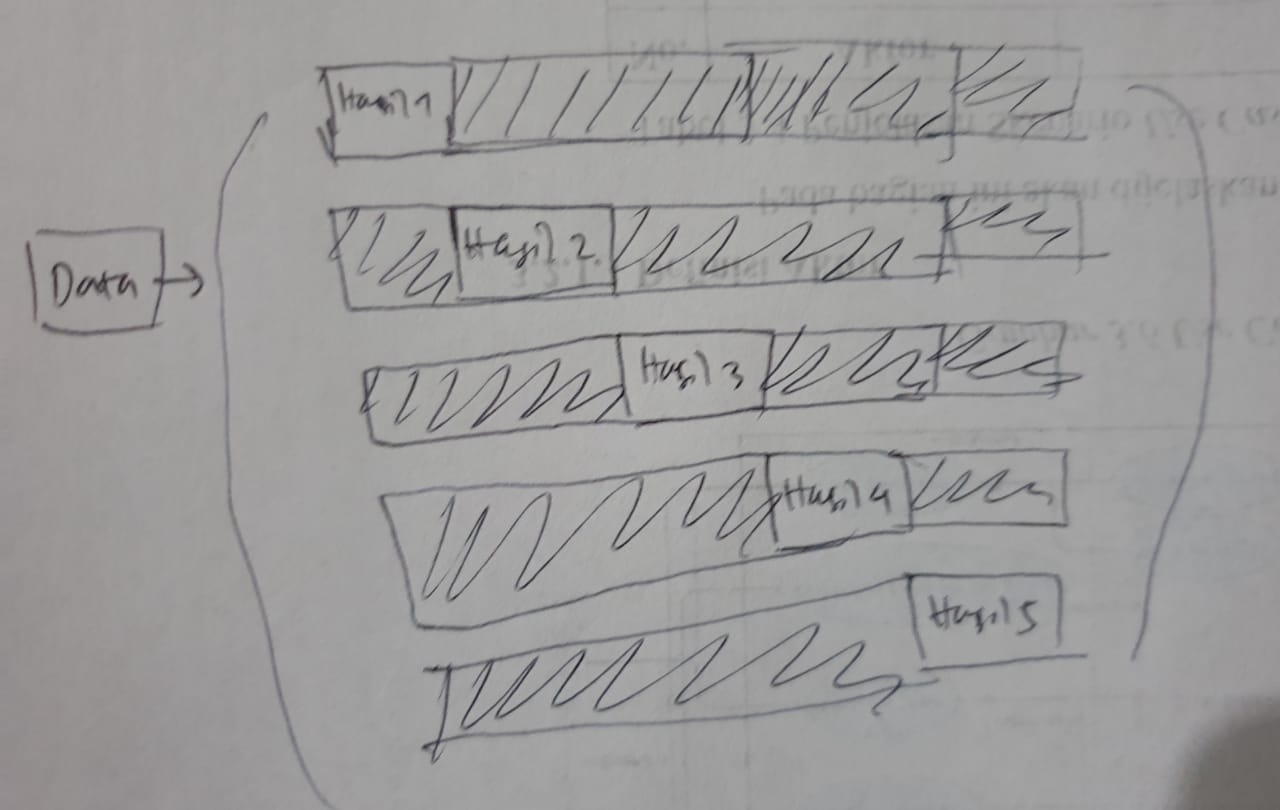
\includegraphics[width=4cm]{figures/1174009/chapter7/teori2.jpeg}
    \centering
      \caption{Ilustrasi  K Fold Cross Validation pada dataset Komentar Youtube}
\end{figure}

\item Jelaskan apa maksudnya kode program \emph{for train, test in splits}
\par Membagi susunan atau matriks menjadi rangkaian acak, dimana data yang dimasukan akan dibagi dengan porsi yang sesuai dengan Train dan Test datanya. untuk lebih jelas tentang bagaimana penggunaannya dapat dilihat pada Gambar

\begin{figure}[H]
    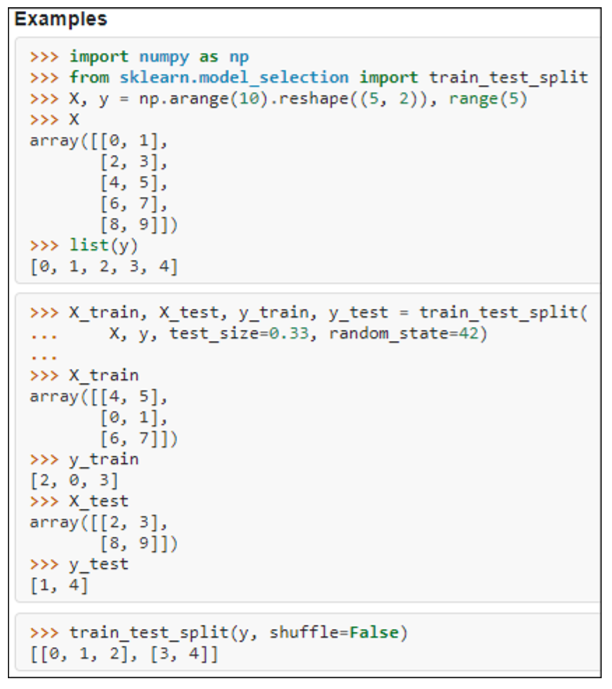
\includegraphics[width=4cm]{figures/1174009/chapter7/teori3.png}
    \centering
      \caption{Ilustrasi  penggunaan Train dan Test Split}
\end{figure}

\item Maksud Code program \emph{train\_content = d['CONTENT'].iloc[train\_idx]} dan \emph{test\_content = d['CONTENT'].iloc[train\_idx]}
\par pada code tersebut dimaksudkan untuk membaca data isian yang terdapat pada kolom yang bernama attributenya CONTENT sebagai data TRAIN dan data TEST, untuk ilustrasinya dapat dilihat pada Gambar

\begin{figure}[H]
    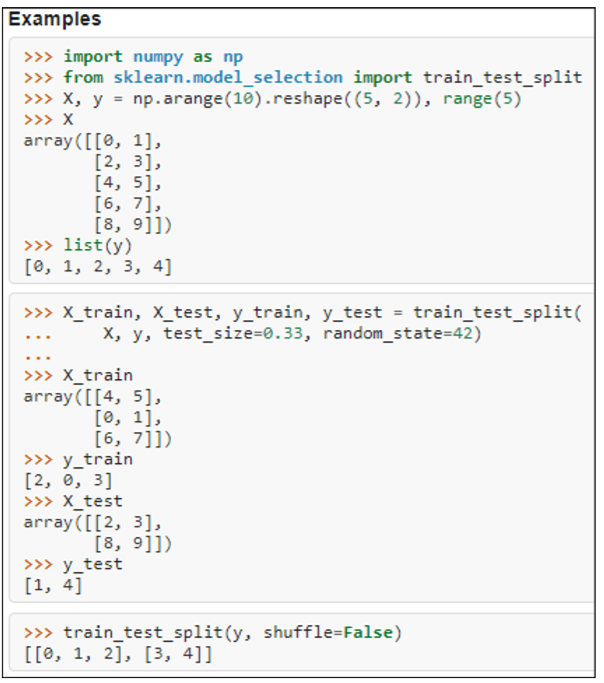
\includegraphics[width=4cm]{figures/1174009/chapter7/teori4.png}
    \centering
      \caption{Ilustrasi  penggunaan Train dan Test Split}
\end{figure}

\item maksud dari fungsi \emph{tokenizer = Tokenizer(num\_words=2000)} dan \emph{tokenizer.fit\_on\_texts(train\_content)}
\par pada code tersebut dimana penggunaan Tokenizer berguna untuk membaca data teks yang berformat kalimat untuk disusun sebanyak 2000 kata, fungsi fit\_on\_texts(train\_content) untuk membaca data Teks Tokenizer tadi untuk dimasukan kedalam kolom CONTENT pada dataset. untuk contoh ilustrasi data yang digunakan dapat dilihat pada Gambar

\begin{figure}[H]
    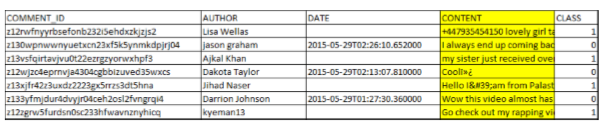
\includegraphics[width=4cm]{figures/1174009/chapter7/teori5.png}
    \centering
      \caption{data Content yang dimaksud}
\end{figure}

\item maksud dari fungsi \emph{d\_train\_inputs = tokenizer.texts\_to\_matrix(train\_content, mode='tfidf')} dan \emph{d\_test\_inputs = tokenizer.texts\_to\_ matrix(test\_content, mode='tfidf')}

\par pada code yang pertama terdapat fungsi yang digunakan untuk mengolah data variable d\_train\_inputs dan d\_test\_inputs dengan menggunakan tokernizer dengan fungsi yang merubah data teks menjadi data matrix dengan pemrosesan datanya sesuai dengan data Variable train\_content dan test\_content dengan metodenya adalah TF-IDF. untuk contoh ilustrasi dari penjelasan tersebut dapat dilihat pada Gambar

\begin{figure}[H]
    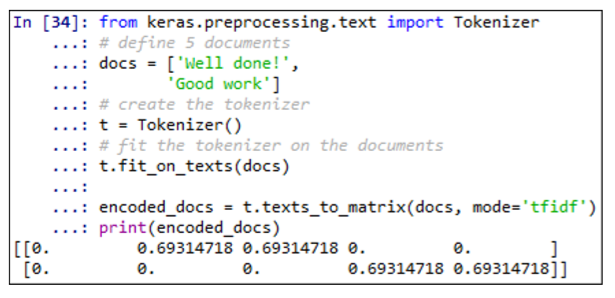
\includegraphics[width=4cm]{figures/1174009/chapter7/teori6.png}
    \centering
      \caption{Contoh code tentang penggunaan texts\_to\_matrix}
\end{figure}

\item maksud dari fungsi \emph{d\_train\_inputs = d\_train\_inputs/np.amax(np.absolute(d\_train\_inputs))} dan \emph{d\_test\_inputs = d\_test\_inputs/np.amax(np.absolute(d\_test\_inputs))}

\par pada code tersebut berfungsi sebagai pengelolaan data Variable d\_train\_inputs dan d\_test\_inputs dengan menggunakan perintah metode yang terdapat pada Library Numpy metode yang diggunakan adalah AMAX yang berguna untuk mengambil nilai maksimum yang terdapat pada data arraynya atau mencari nilai maksimum dari panjang sumbu yang terproses dan ABSOLUTE yang berguna untuk untuk mengkalkulasi nilai pasti dari setiap data elemennya. untuk contoh dari pengguaan AMAX dan ABSOLUTE dapat dilihat pada Gambar

\par berikut ini adalah contoh Code yang digunakan untuk menjelaskan penggunaan AMAX :
\begin{figure}[H]
    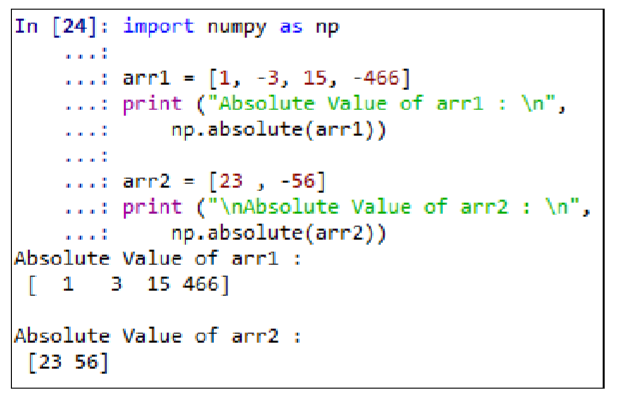
\includegraphics[width=4cm]{figures/1174009/chapter7/teori7.png}
    \centering
      \caption{penggunaan Numpy AMAX}
\end{figure}

\par berikut ini adalah contoh Code yang digunakan untuk menjelaskan penggunaan ABSOLUTE :
\begin{figure}[H]
    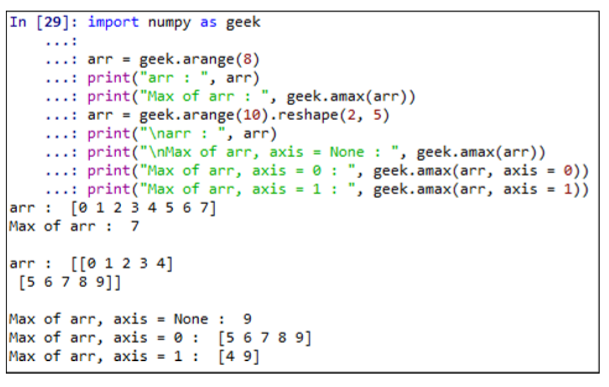
\includegraphics[width=4cm]{figures/1174009/chapter7/teori8.png}
    \centering
      \caption{penggunaan Numpy ABSOLUTE}
\end{figure}

\item maksud fungsi dari \emph{d\_train\_outputs = np\_utils.to\_categorical(d['CLASS'].iloc[train\_idx])} dan \emph{d\_test\_outputs = np\_utils.to\_categorical(d['CLASS'].iloc[test\_idx])} dalam kode program

\par pada code tersebut menjelaskan penggunaan Library Numpy yang akan mengelola data d\_train\_outputs dan d\_test\_outputs dengan menggunakan perintah atau metode TO\_CATEGORICAL dimana data yang diambil adalah data CLASS dengan index data yang dituju adalah train\_idx dan test\_idx, dimana to\_categorical berguna untuk mengkonversikan data kelas Vektor(Integer) menjadi data kelas Binary Matrix. contoh penggunaan to categorical dapat dilihat pada Gambar

\begin{figure}[H]
    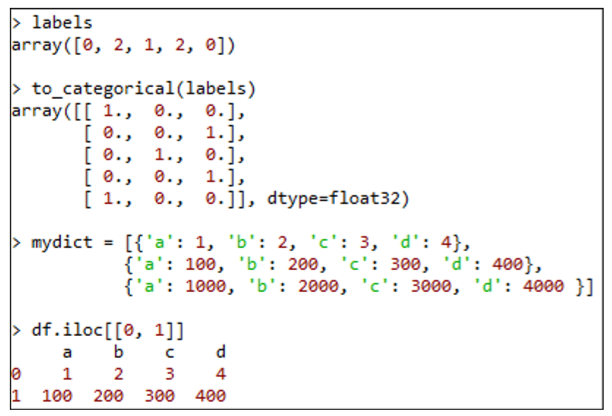
\includegraphics[width=4cm]{figures/1174009/chapter7/teori9.png}
    \centering
      \caption{Contoh Code dan Hasil dari penggunaan to\_categorical dan iloc}
\end{figure}

\item Penjelasan pada fungsi code dengan Ilustrasi Neural Networknya
\begin{lstlisting}[caption=Membuat model Neural Network,label={lst:3}]
       model = Sequential()
       model.add(Dense(512, input_shape=(2000,)))
       model.add(Activation('relu'))
       model.add(Dropout(0.5))
       model.add(Dense(2))
       model.add(Activation('softmax'))
\end{lstlisting}
\par pada code yang terdapat pada  Listing \ref{lst:3}, dijelaskan bahwa dibuatkannya Variable 'model' untuk menampung model Sequential() atau metode yang berguna untuk menumpuk data Linear. berikut ini adalah  penjelasan dari masing - masing fungsi yang terdapat pada Code tersebut :
\begin{itemize}
\item Dense (512, input\_shape = (2000,)) dan (2)
\par dimana data yang diolah akan berjumlah 512 dengan shape yang diolah dalah 2000 begitu juga dengan yang 2

\item Activation ('relu') dan ('softmax')
\par Activation adalah untuk melakukan penggunaan fungsi matematika, relu yang berarti fungsi dari metode 'Rectified Linear Unit' dan softmax yang berguna untuk menghasilkan data Vector yang merepresentasikan nilai distibusi probabilitas dari daftar nl=ilai output yang memiliki potensi.

\item Dropout(0.5)
\par melakukan set sebanyak 50 persen pada output atau nilai hasil yang dikeluarkan dari pengelolaan data pada visible layer dan hidden layer.
\end{itemize}
\par berikut ini adalah contoh dari struktur Neural Network yang terjadi :
\begin{figure}[H]
    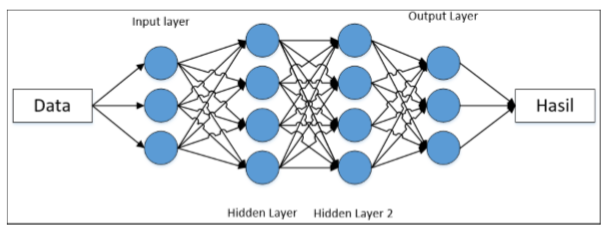
\includegraphics[width=4cm]{figures/1174009/chapter7/teori10.png}
    \centering
      \caption{Contoh dari struktur Neural Network yang terjadi}
\end{figure}

\item Maksud dari fungsi pada Code berikut :
\begin{lstlisting}[caption=Compile model,label={lst:4}]
	model.compile(loss='categorical_crossentropy', optimizer='adamax',
	                  metrics=['accuracy'])
\end{lstlisting}
\par pada code di Listing \ref{lst:4} menjelaskan tentang proses yang berlangsung untuk menampilkan nilai LOSS dan ACCURACY yang dihasilkan dari Compile pada program diatas.

\item Jelaskan apa itu Deep Learning
\par Deep Learning adalah rangkaian metode untuk bisa melatih jaringan saraf buatan multi lapisan atau mempunyai banyak lapisan. Metode ini sangat efektif dan lebih mudah dalam mengidentifikasi pola dari data yang dimasukkan. Deep Learning juga dapat meningkatkan bagian AI, mulai dari memproses bahasa alami yang kita katakana sampai dengan mengambil gambar. Oleh karena itu Deep Learning merupakan otak yang lebih baik dan unggul untuk meningkatkan cara kerja pada sistem komputer

\item Jelaskan Apa itu Deep Neural Network dan apa perbedaanya dengan Deep Learning
\par Deep Neural Network adalah Neural Network dengan tingkat kompleksitas tertentu, Neural Network dengan lebih dari dua lapisan.  Neural Network dalam menggunakan pemodelan matematika yang canggih untuk memproses data dengan cara yang kompleks. perbedaan antara Deep Learning dan DNN adalah DNN merupakan sebuah Algoritma yang terdapat dalam Deep Learning itu sendiri sedangkan Deep Learning adalah sebuah pengguna dari algoritma pada DNN.

\item Jelaskan dengan ilustrasi gambar buatan sendiri(langkah per langkah) bagaimana perhitungan algoritma konvolusi dengan ukuran stride (NPM mod3+1) x (NPM mod3+1) yang terdapat max pooling

\par Konvolusi terdapat pada operasi pengolahan citra yang mengalikan sebuah citra dengan sebuah mask atau kernel, Stride adalah parameter yang berfungsi untuk menentukan pergeseran pada filter data pixel yang terjadi. untuk contoh penggunaannya dapat dilihat pada Gambar

\begin{figure}[H]
    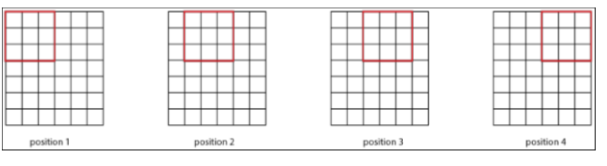
\includegraphics[width=4cm]{figures/1174009/chapter7/teori11.png}
    \centering
      \caption{Penggunaan Konvolusi dengan Stridenya adalah 3 x 3}
\end{figure}

\end{enumerate}


\subsection{Pemrograman}
\begin{enumerate}

\item No. 1 Kode Program Blok \# In 1
\par \lstinputlisting[firstline=1, lastline=4]{src/1174009/chapter7/MathSymbols.py}
Keterangannya sebagai berikut :
\begin{itemize}
\item Melakukan Import Library CSV
\item Melakukan Import Library PIL (Python Imaging Library) yang berguna untuk melakukan pemrosesan data yang bersifat Image. dengan fungsi yang diimport adalah pil\_image
\item Melakukan Import data preprocessing dari Library Keras yang akan memproses data Image.
\item hasilnya dapat dilihat pada Gambar 
\begin{figure}[H]
    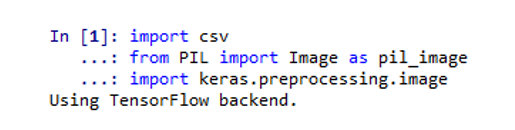
\includegraphics[width=4cm]{figures/1174009/chapter7/1.png}
    \centering
    \caption{kode program pada blok  In[1].}
    \end{figure}
\end{itemize}



\item No. 2 Kode Program Blok \# In 2
\par \lstinputlisting[firstline=6, lastline=20]{src/1174009/chapter7/MathSymbols.py}
Keterangannya sebagai berikut :
\begin{itemize}
\item Membuat Variable 'imgs' dan 'classes' yang memiliki nilai array kosong agar dapat diisikan oleh data nantinya.
\item Membuka file csv dari Folder HSYv2 dengan nama file hasy-data-labels.csv yang dialiaskan sebagai Variable csvfile.
\item Variabel csvreader akan menggunakan fungsi reader pada library csv untuk membaca file pada variable csvfile.
\item Membuat Variable i yang bernilai NOL.
\item Membuat pemrosesan data yang akan membaca datan dari csvreader dengan membuat Variable 'row', dimasukan dengan fungsi IF jika i lebih besar dari NOL.
\item membuat Variable 'img' yang berisi data pemrosesan Library keras dengan fungsi image.im\_to\_array yang akan mmebuat data yang dibuka menjadi format array pada Folder HASYv2 yang dimulai dari NOL.
\item Hasil dari variabel img akan dibagi dengan 255.0
\item .append akan membuat list array baru untuk baris 0 baris 2 pada img.
\item Menyimpan setiap class nya  pada baris 2
\item Penambahan i sebanyak 1. 
\item hasilnya dapat dilihat pada Gambar
\begin{figure}[H]
    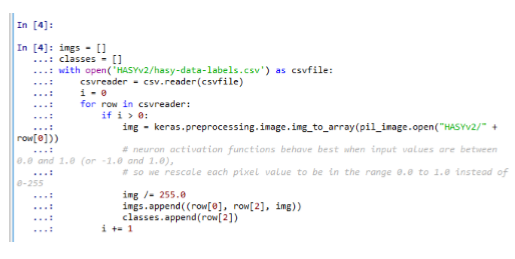
\includegraphics[width=4cm]{figures/1174009/chapter7/2.png}
    \centering
    \caption{kode program pada blok  In[2].}
    \end{figure}
\end{itemize}



\item No. 3 Kode Program Blok \# In 3
\par \lstinputlisting[firstline=22, lastline=27]{src/1174009/chapter7/MathSymbols.py}
Keterangannya sebagai berikut :
\begin{itemize}
\item Melakukan Import Library random.
\item Membuat parameter dari penggunaan library random yang akan mengacak data dengan fungsi 'shuffle' pada data Variable 'imgs'.
\item Membagi index data dari imgs dengan cara mengalikan 80\% dengan jumlah data dari imgs.
\item Untuk data train mengambil hasil dari perhitungan sebelumnya.
\item Untuk data test mengambil sisa dari jumlah yang telah dijadikan data train.
\item hasil dapat dilihat pada Gambar'
\begin{figure}[H]
    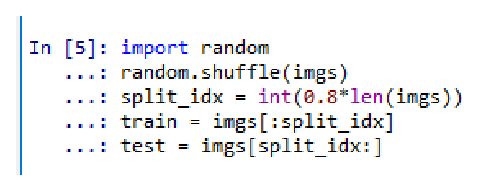
\includegraphics[width=4cm]{figures/1174009/chapter7/3.png}
    \centering
    \caption{kode program pada blok  In[3].}
    \end{figure}
\end{itemize}


\item No. 4 Kode Program Blok \# In 4
\par \lstinputlisting[firstline=29, lastline=36]{src/1174009/chapter7/MathSymbols.py}
Keterangannya sebagai berikut :
\begin{itemize}
\item Melakukan Import dari Library Numpy dialiaskan menjadi np.
\item Variabel train\_input mengubah input menjadi sebuah array yang diambil dari baris 2, dari data train.
\item Variabel test\_input mengubah input menjadi sebuah array yang diambil dari baris 2, dari data test.
\item Variabel train\_output mengubah input menjadi sebuah array yang diambil dari baris 1, dari data train.
\item Variabel train\_output mengubah input menjadi sebuah array yang diambil dari baris 1, dari data test.
\item hasil dapat dilihat pada Gambar
\begin{figure}[H]
    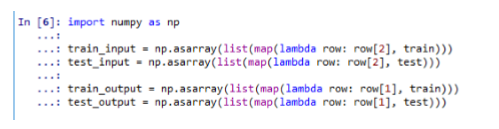
\includegraphics[width=4cm]{figures/1174009/chapter7/4.png}
    \centering
    \caption{kode program pada blok  In[4].}
    \end{figure}
\end{itemize}



\item No. 5 Kode Program Blok \# In 5
\par \lstinputlisting[firstline=38, lastline=40]{src/1174009/chapter7/MathSymbols.py}
Keterangannya sebagai berikut :
\begin{itemize}
\item Melakukan Import fungsi Labeldari Library sklearn 
\item Melakukan Import fungsi OneHotEncoderdari Library sklearn
\item hasil dapat dilihat pada Gambar
\begin{figure}[H]
    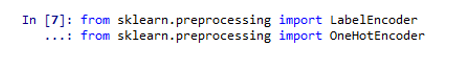
\includegraphics[width=4cm]{figures/1174009/chapter7/5.png}
    \centering
    \caption{kode program pada blok  In[5].}
    \end{figure}
\end{itemize}



\item No. 6 Kode Program Blok \# In 6
\par \lstinputlisting[firstline=42, lastline=45]{src/1174009/chapter7/MathSymbols.py}
Keterangannya sebagai berikut :
\begin{itemize}
\item Membuat Variabel label\_encoder yang akan memanggil fungsi LabelEncoder tadi.
\item Membuat Variabel integer\_encoded yang akan menggunakan labelencoder untuk melakukan fit pada classes agar berubah datanya menjadi integer.
\item hasil dapat dilihat pada Gambar
\begin{figure}[H]
    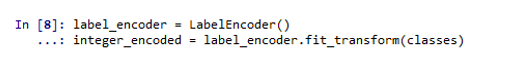
\includegraphics[width=4cm]{figures/1174009/chapter7/6.png}
    \centering
    \caption{kode program pada blok  In[6].}
    \end{figure}
\end{itemize}



\item No. 7 Kode Program Blok \# In 7
\par \lstinputlisting[firstline=47, lastline=50]{src/1174009/chapter7/MathSymbols.py}
Keterangannya sebagai berikut :
\begin{itemize}
\item Membuat Variabel onehot\_encoder akan memanggil fungsi OneHotEncoder dimana tidak berisikan matriks sparse.
\item Pada variabel integer\_encoded akan diubah bentuknya dimana setiap nilai integer akan direpresentasikan sebagai vektor binari dengan nilai 0 kecuali index dari integer tersebut ditandai dengan 1.
\item Melakukan fit untuk one hot encoder kedalam integer\_encoder.
\item hasil dapat dilihat pada Gambar
\begin{figure}[H]
    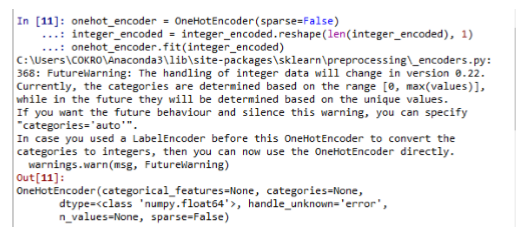
\includegraphics[width=4cm]{figures/1174009/chapter7/7.png}
    \centering
    \caption{kode program pada blok  In[7].}
    \end{figure}
\end{itemize}



\item No. 8 Kode Program Blok \# In 8
\par \lstinputlisting[firstline=52, lastline=59]{src/1174009/chapter7/MathSymbols.py}
Keterangannya sebagai berikut :
\begin{itemize}
\item Membuat Variabel train\_output\_int  akan mengubah data dari train\_output menjadi LabelEncoder
\item Membuat Variable train\_output dimana setelah diubah labelnya menjadi integer dilakukan onehot\_encoding diambil dari train\_output\_int dan menggunakan .reshape untuk memberikan bentuk baru ke array tanpa mengubah datanya dengan keterangan jika index dari integer tersebut ditandai dengan 1 dan sisanya yang bukan nol.
\item Membuat Variabel test\_output\_int  akan mengubah data dari test\_output menjadi LabelEncoder
\item Membuat Variable test\_output dimana setelah diubah labelnya menjadi integer dilakukan one hot encoding diambil dari test\_output\_int dan menggunakan .reshape untuk memberikan bentuk baru ke array tanpa mengubah datanya dengan keterangan jika index dari integer tersebut ditandai dengan 1 dan sisanya yang bukan nol.
\item Membuat Variabel num\_classes akan menampilakn jumlah data dari classes yang telah dilakukan label encoder
\item Melakukan print dengan Format tulisannya adalah "Number of classes : \%d dmana mengembalikan nilai integer dari num\_classes.
\item hasil dapat dilihat pada Gambar
\begin{figure}[H]
    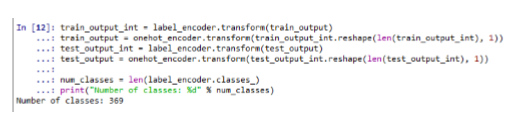
\includegraphics[width=4cm]{figures/1174009/chapter7/8.png}
    \centering
    \caption{kode program pada blok  In[8].}
    \end{figure}
\end{itemize}



\item No. 9 Kode Program Blok \# In 9
\par \lstinputlisting[firstline=61, lastline=64]{src/1174009/chapter7/MathSymbols.py}
Keterangannya sebagai berikut :
\begin{itemize}
\item Melakukan Import Sequential dari model pada Library Keras.
\item Melakukan Import Dense, Dropout, Flatten dari modul Layers pada Library Keras.
\item Melakukan Import Conv2D, MaxPooling2D dari modul Layers pada Library Keras.
\item hasil dapat dilihat pada Gambar
\begin{figure}[H]
    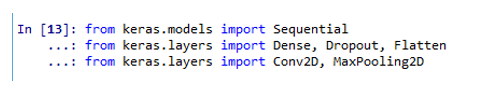
\includegraphics[width=4cm]{figures/1174009/chapter7/9.png}
    \centering
    \caption{kode program pada blok  In[9].}
    \end{figure}
\end{itemize}

\item No. 10 Kode Program Blok \# In 10
\par \lstinputlisting[firstline=66, lastline=81]{src/1174009/chapter7/MathSymbols.py}
Keterangannya sebagai berikut :
\begin{itemize}
\item Melakukan pemodelan Sequential.
\item Menambahkan Konvolusi 2D dengan 32 filter konvolusi masing-masing berukuran 3x3 dengan algoritam activation relu dengan data dari train\_input mulai dari baris nol.
\item Menambahkan Max Pooling dengan matriks 2x2.
\item Dilakukan lagi penambahkan Konvolusi 2D dengan 32 filter konvolusi masing-masing berukuran 3x3 dengan algoritam activation relu.
\item Menambahkan lagi Max Pooling dengan matriks 2x2.
\item Mendefinisikan inputan dengan 1024 neuron dan menggunakan algoritma tanh untuk activationnya.
\item Dropout terdiri dari pengaturan secara acak tingkat pecahan unit input ke 0 pada setiap pembaruan selama waktu pelatihan, yang membantu mencegah overfitting sebesar 50\% .
\item Untuk output layer menggunakan data dari variabel num\_classes dengan fugsi activationnya softmax.
\item Mengonfigurasi proses pembelajaran, yang dilakukan melalui metode compile,sebelum melatih suatu model.
\item Menampilkan atau mencetak representasi ringkasan model yang telah dibuat.
\begin{figure}[H]
    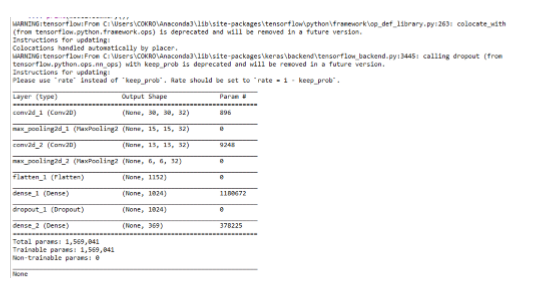
\includegraphics[width=4cm]{figures/1174009/chapter7/10.png}
    \centering
    \caption{kode program pada blok  In[10].}
    \end{figure}
\end{itemize}


\item No. 11 Kode Program Blok \# In 11
\par \lstinputlisting[firstline=83, lastline=85]{src/1174009/chapter7/MathSymbols.py}
Keterangannya sebagai berikut :
\begin{itemize}
\item Impor Modul Callbacks dari Librari Keras.
\item Variabel callback mendefinisikan Callback ini untuk menulis log untuk TensorBoard, yang memungkinkan Anda untuk memvisualisasikan grafik dinamis dari pelatihan dan metrik pengujian Anda, serta histogram aktivasi untuk berbagai lapisan dalam model Anda.
\begin{figure}[H]
    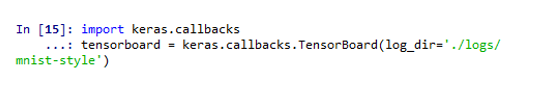
\includegraphics[width=4cm]{figures/1174009/chapter7/11.png}
    \centering
    \caption{kode program pada blok  In[11].}
    \end{figure}
\end{itemize}

\item No. 12 Kode Program Blok \# In 12
\par \lstinputlisting[firstline=87, lastline=97]{src/1174009/chapter7/MathSymbols.py}
Keterangannya sebagai berikut :
\begin{itemize}
\item Melakukan fit model dengan 32 ukuran subset dari sampel pelatihan Anda
\item Epoch sebanyak 10 kali
\item Vebrose=2 maksudnya menampilkan nomor dari epoch yang sedang berjalan atau yang sudah dijalankan.
\item Validasi plit sebanayk 20\% sebagai fraksi data pelatihan untuk digunakan sebagai data validasi.
\item Menggunakan TensorBoard sebagai callback untuk diterapkan selama pelatihan dan validasi.
\item Variabel score mengembalikan nilai evaluate untuk menampilkan data lost dan data accuracy dari test
\item Menampilkan data loss dengan menghitung jumlah kemunculan nol .
\item Menampilkan data accuracy dengan menghitung jumlah kemunculan 1.
\begin{figure}[H]
    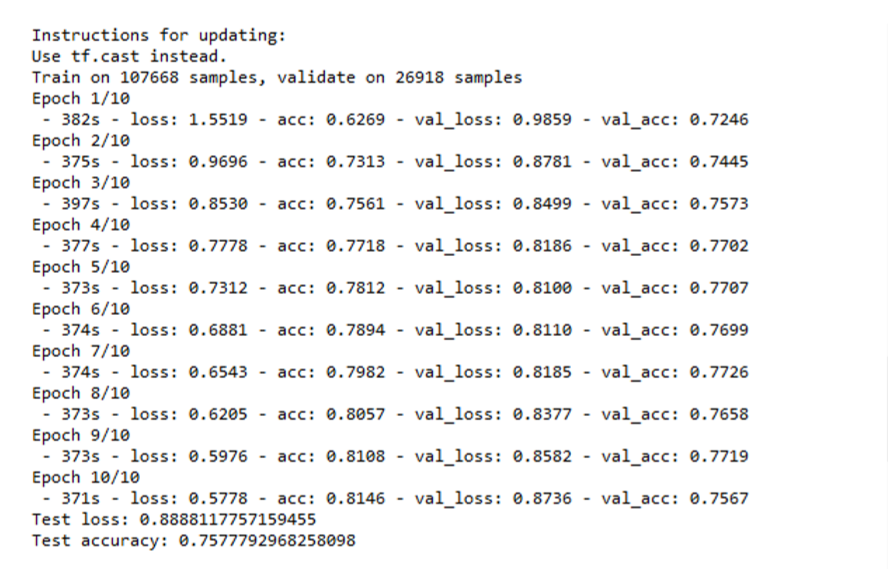
\includegraphics[width=4cm]{figures/1174009/chapter7/12.png}
    \centering
    \caption{kode program pada blok  In[12].}
    \end{figure}
\end{itemize}

\item No. 13 Kode Program Blok \# In 13
\par \lstinputlisting[firstline=99, lastline=131]{src/1174009/chapter7/MathSymbols.py}
Keterangannya sebagai berikut :
\begin{itemize}
\item impor modul time dari python anaconda
\item Variabel result berisikan array kosong.
\item Menggunakan convolution 2D yang dimana akan memiliki 1 atau 2 layer.
\item Mendefinisikan dense\_size dengan ukuran 128, 256, 512, 1024, 2048
\item Mendefinsikan drop\_out dengan 0, 25\%, 50\%, dan 75\%
\item Melakukan pemodelan Sequential
\item Jika ini adalah layer pertama, kita perlu memasukkan bentuk input.
\item Kalau tidak kita hanya akan menambahkan layer.
\item Kemudian, setelah menambahkan layer konvolusi, kita akan melakukan hal yang sama dengan max pooling.
\item  Lalu, kita akan meratakan atau flatten dan menambahkandense size ukuran apa pun yang berasal dari dense\_size. Dimana akan selalu menggunakan algoritma tanh
\item Jika dropout digunakan, kita akan menambahkan layer dropout. Menyebut dropout ini berarti, katakanlah 50\%, bahwa setiap kali ia memperbarui bobot setelah setiap batch, ada peluang 50\% untuk setiap bobot yang tidak akan diperbarui
\item menempatkan ini di antara dua lapisan padat untuk dihidupkan dari melindunginya dari overfitting.
\item  Lapisan terakhir akan selalu menjadi jumlah kelas karena itu harus, dan menggunakan softmax. Itu dikompilasi dengan cara yang sama.
\item Atur direktori log yang berbeda untuk TensorBoard sehingga dapat membedakan konfigurasi yang berbeda.
\item Variabel start akan memanggil modul time atau waktu
\item Melakukan fit atau compile 
\item MElakukan scoring dengan .evaluate yang akan menampilkan data loss dan accuracy dari model
\item end merupakan variabel untuk melihat waktu akhir pada saat pemodelan berhasil dilakukan.
\item Menampilkan hasil dari run skrip diatas
\begin{figure}[H]
    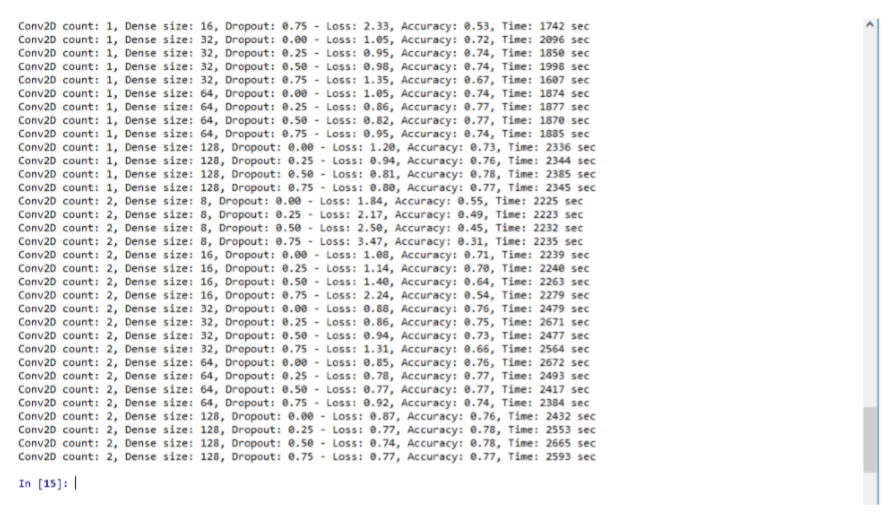
\includegraphics[width=4cm]{figures/1174009/chapter7/13.png}
    \centering
    \caption{kode program pada blok  In[13].}
    \end{figure}
\end{itemize}

\item No. 14 Kode Program Blok \# In 14
\par \lstinputlisting[firstline=134, lastline=145]{src/1174009/chapter7/MathSymbols.py}
Keterangannya sebagai berikut :
\begin{itemize}
\item Melakukan pemodelan Sequential
\item Untuk layer pertama, Menambahkan Convolutio 2D dengan dmensi 32, dan ukuran matriks 3x3 dengan function aktivasi yang digunakan yaitu relu dan menampilkan input\_shape
\item Dilakukan Max Pooling 2D dengan ukuran matriks 2x2
\item Untuk layer kedua, melakukan Convolusi lagi dengan kriteria yang sama tanpa menambahkan input, ini dilakukan untuk mendapatkan data yang terbaik
\item Flatten digubakan ntuk meratakan inputan
\item Menambahkan dense input sebanyak 128 neuron dengan menggunakan function aktivasi tanh.
\item Dropout sebanyak 50\% untuk menghindari overfitting
\item Menambahkan dense pada model untuk output dimana layer ini akan menjadi jumlah dari class yang ada.
\item Mengcompile model yang didefinisikan diatas
\item Menampilkan ringkasan dari pemodelan yang dilakukan
\begin{figure}[H]
    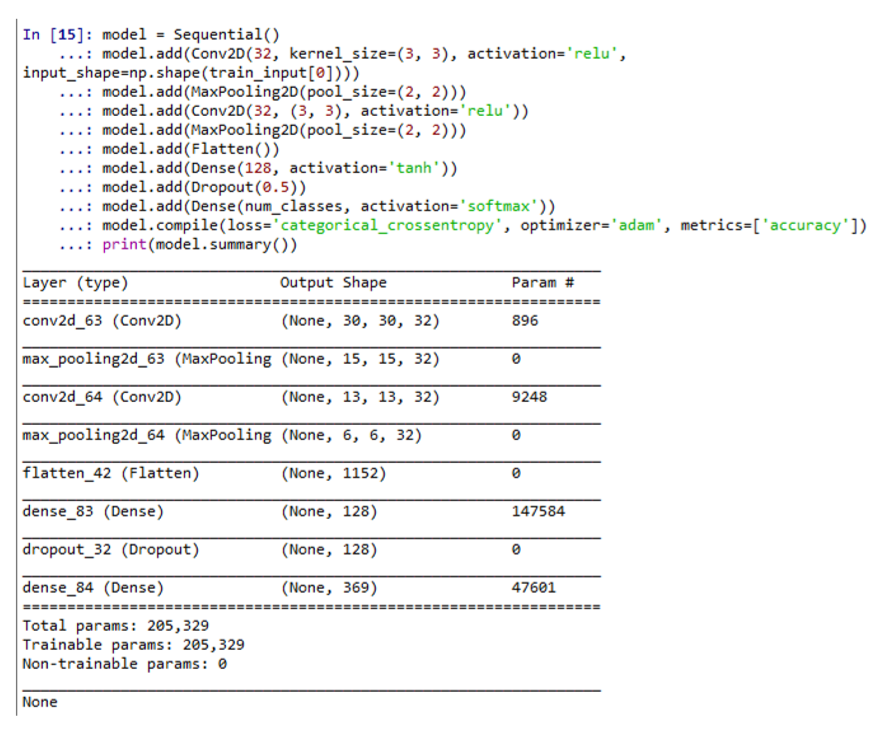
\includegraphics[width=4cm]{figures/1174009/chapter7/14.png}
    \centering
    \caption{kode program pada blok  In[14].}
    \end{figure}
\end{itemize}

\item No. 15 Kode Program Blok \# In 15
\par \lstinputlisting[firstline=147, lastline=150]{src/1174009/chapter7/MathSymbols.py}
Keterangannya sebagai berikut :
\begin{itemize}
\item Melakukan fit dengan join data train dan test agar dapat dilakukan pelatihan untuk jaringan pada smeua data yang dimiliki.
\begin{figure}[H]
    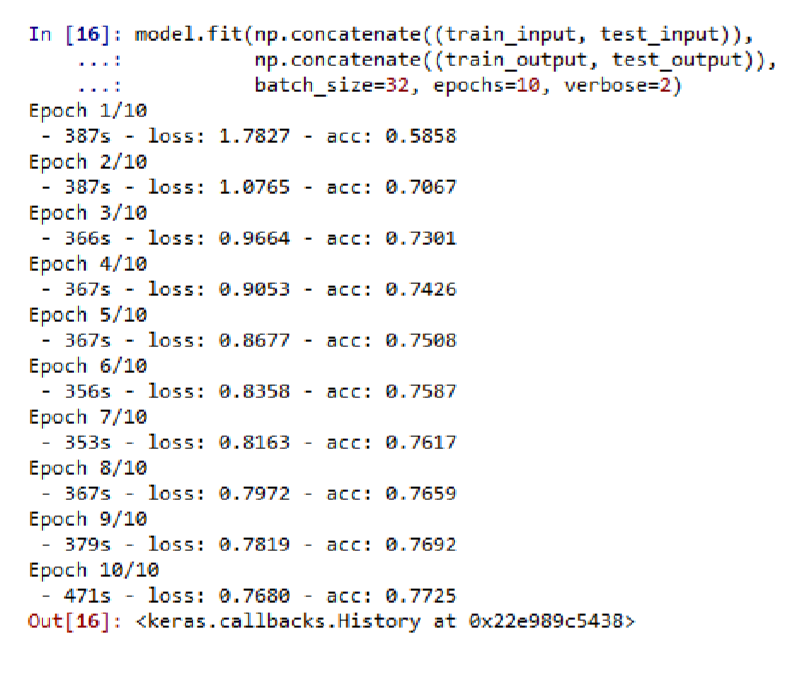
\includegraphics[width=4cm]{figures/1174009/chapter7/15.png}
    \centering
    \caption{kode program pada blok  In[15].}
    \end{figure}
\end{itemize}

\item No. 16 Kode Program Blok \# In 16
\par \lstinputlisting[firstline=152, lastline=153]{src/1174009/chapter7/MathSymbols.py}
Keterangannya sebagai berikut :
\begin{itemize}
\item Menyimpan atau save model yang telah di latih dengan nama mathsymbols.model 
\begin{figure}[H]
    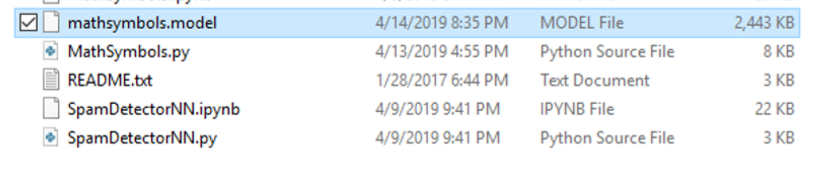
\includegraphics[width=4cm]{figures/1174009/chapter7/16.png}
    \centering
    \caption{kode program pada blok  In[16].}
    \end{figure}
\end{itemize}

\item No. 17 Kode Program Blok \# In 17
\par \lstinputlisting[firstline=155, lastline=156]{src/1174009/chapter7/MathSymbols.py}
Keterangannya sebagai berikut :
\begin{itemize}
\item Simpan label enkoder (untuk membalikkan one-hot encoder) dengan nama classes.npy
\begin{figure}[H]
    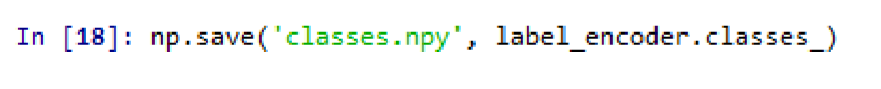
\includegraphics[width=4cm]{figures/1174009/chapter7/17.png}
    \centering
    \caption{kode program pada blok  In[17].}
    \end{figure}
\end{itemize}

\item No. 18 Kode Program Blok \# In 18
\par \lstinputlisting[firstline=159, lastline=163]{src/1174009/chapter7/MathSymbols.py}
Keterangannya sebagai berikut :
\begin{itemize}
\item Impor models dari librari Keras
\item Variabel model2 akan memanggil model yang telah disave tadi 
\item Menampilkan ringkasan dari hasil pemodelan
\begin{figure}[H]
    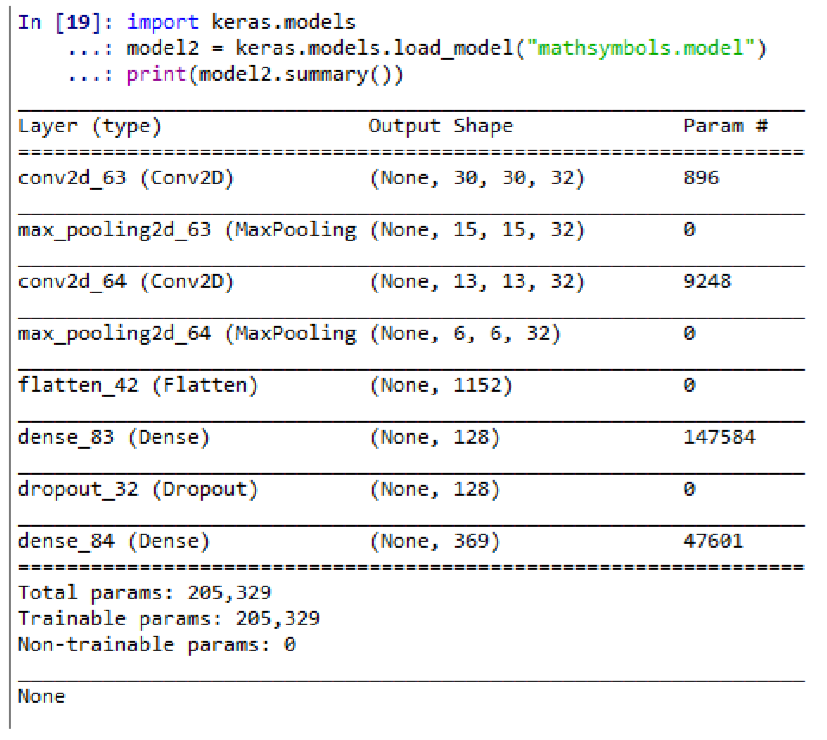
\includegraphics[width=4cm]{figures/1174009/chapter7/18.png}
    \centering
    \caption{kode program pada blok  In[18].}
    \end{figure}
\end{itemize}

\item No. 19 Kode Program Blok \# In 19
\par \lstinputlisting[firstline=165, lastline=178]{src/1174009/chapter7/MathSymbols.py}
Keterangannya sebagai berikut :
\begin{itemize}
\item Memanggil fungsi LabelEncoder
\item Variabel label\_encoder akan memanggil class yang disave sebelumnya.
\item Function Predict akan mengubah gambar kedalam bentuk array
\item Variabel prediction akan melakukan prediksi untuk model2 dengan reshape variabel newimg dengan bentukarray 4D.
\item Variabel inverted akan mencari nilai tertinggi output dari hasil prediksi tadi
\item Menampilkan hasil dari variabel prediction dan inverted
\begin{figure}[H]
    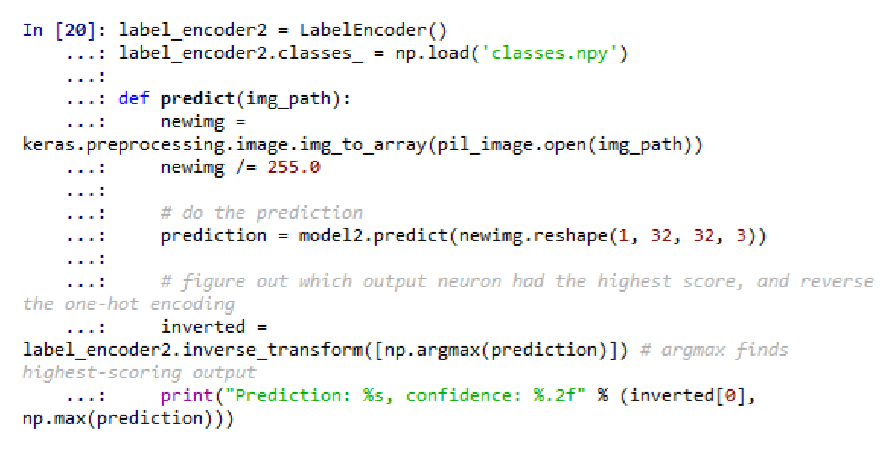
\includegraphics[width=4cm]{figures/1174009/chapter7/19.png}
    \centering
    \caption{kode program pada blok  In[19].}
    \end{figure}
\end{itemize}

\item No. 20 Kode Program Blok \# In 20
\par \lstinputlisting[firstline=180, lastline=185]{src/1174009/chapter7/MathSymbols.py}
Keterangannya sebagai berikut :
\begin{itemize}
\item Melakukan prediksi dari pelatihan dari gambar v2-00010.png
\item Melakukan prediksi dari pelatihan dari gambar v2-00500.png
\item Melakukan prediksi dari pelatihan dari gambar v2-00700.png
\begin{figure}[H]
    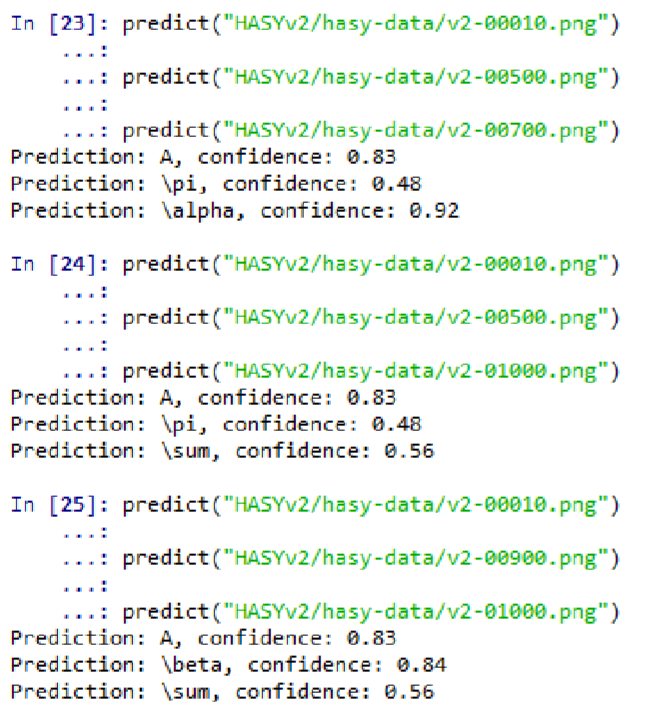
\includegraphics[width=4cm]{figures/1174009/chapter7/20.png}
    \centering
    \caption{kode program pada blok  In[20].}
    \end{figure}
\end{itemize}

\end{enumerate}